\documentclass[a4paper,11pt]{article}

\usepackage[top=2.4cm,
            bottom=2.4cm,
            left=2.8cm,
            right=2.8cm]{geometry}
\usepackage[english]{babel}
\usepackage[utf8]{inputenc}
\usepackage[T1]{fontenc}
\usepackage{amsmath}
\usepackage{graphicx}
\usepackage{float}
\usepackage[english]{varioref}
\usepackage{hyperref}
\usepackage{url}
\usepackage[font=small,labelfont=bf]{caption}
\usepackage{framed}
\usepackage{quoting}
\usepackage{subcaption}
\usepackage[dvipsnames]{xcolor}

% for ChatGPT
\newenvironment{shadedquotation1}
    {\colorlet{shadecolor}{JungleGreen!15}\begin{shaded*}
    \quoting[leftmargin=1cm, rightmargin=1cm, vskip=0pt]
    }
    {\endquoting
    \end{shaded*}
}
% for Bard
\newenvironment{shadedquotation2}
    {\colorlet{shadecolor}{Cerulean!15}\begin{shaded*}
    \quoting[leftmargin=1cm, rightmargin=1cm, vskip=0pt]
    }
    {\endquoting
    \end{shaded*}
}
% for Copilot
\newenvironment{shadedquotation3}
    {\colorlet{shadecolor}{Purple!15}\begin{shaded*}
    \quoting[leftmargin=1cm, rightmargin=1cm, vskip=0pt]
    }
    {\endquoting
    \end{shaded*}
}

\usepackage{tocloft}
% Center the toc index title
\renewcommand\cfttoctitlefont{\hfill\Large\bfseries}
\renewcommand\cftaftertoctitle{\hfill\mbox{}}
% Adjust the width between the titles and page numbers
\cftsetindents{section}{3cm}{2em}
\cftsetindents{subsection}{4cm}{2em}
% C center the titles
\renewcommand{\cftsecleader}{\cftdotfill{\cftdotsep}}
\renewcommand{\cftsecafterpnum}{\hspace*{3cm}\mbox{}\par}
\renewcommand{\cftsubsecleader}{\cftdotfill{\cftdotsep}}
\renewcommand{\cftsubsecafterpnum}{\hspace*{3cm}\mbox{}\par}


\title{\Huge Project Report}
\author{Vignotto Lara -- 111794}
\date{\today}


\begin{document}

\maketitle
\vspace{1cm}
\tableofcontents
\vspace{3.2cm}



%%%%%%%%%%%%%%%%%%%%%%
\section{Introduction}
In this report, I will illustrate how I generated a short comic book story exploiting free online generative AI tools. The document is divided into the following sections:
\begin{itemize}
    \item Tools and Methods: I will describe the AI tools and methods I used to generate the story;
    \item The Story -- Plot and Text: I will present the story, how I generated the text, and the limitations I encountered;
    \item The Art -- Images: I will describe how I generated the illustrations and the limitations and biases of the AI tools I used;
    \item Conclusions: I will draw some conclusions and discuss the results.
\end{itemize}
At the end of this document, there are two appendices: the first one contains the original prompts I used to generate the story, and the second one contains the original prompts I used to generate the illustrations.



%%%%%%%%%%%%%%%%%%%%%%
\section{Tools and Methods}
I used two generative AI tools to generate the story and the illustrations. For the story, I used ChatGPT 3.5 \cite{gpt}, a conversational AI model developed by OpenAI. For the illustrations, I used DALL-E 3 integrated into Microsoft Copilot \cite{copilot2023}, a generative model developed by OpenAI and Microsoft. 
ChatGPT is an AI language model based on OpenAI's GPT (Generative Pre-trained Transformer) architecture. DALL-E 3 is also built upon OpenAI's GPT architecture, but it is specialized for image generation tasks. 

I initially also tried to use other generative AI tools, such as Google Bard \cite{bard} and Microsoft Copilot to generate the story, and DreamStudio \cite{dreamstudio} to generate the illustrations. However, I found that ChatGPT and DALL-E 3 were the most effective tools for my purposes. I will talk about the limitations of these tools in the next sections.

To paginate the comic book, I used \LaTeX, a typesetting system that is widely used for technical and scientific documents. I used the \texttt{tikz} package to create the comic book layout and the \texttt{graphicx} package to include the images.

All the code I used to write this report and paginate story and the illustrations is available on my GitHub repository \cite{github}.



%%%%%%%%%%%%%%%%%%%%%%
\section{The Story -- Plot and Text}

The story is a science fiction tale set in a future where humanity lives in an arcology, a massive, self-sustaining structure that houses communities and ecosystems. The protagonist is Dr.~Evelyn Hayes, a communication scientist devoted to her work within the arcology. One day, she receives a mysterious message from an unknown source. Her young daughter seems to possess an intuition that the message is a cry for help from a distant planet. Dr.~Hayes decides to investigate the message and embarks on a journey to the planet. 

The story is intended as a pilot episode, and could be expanded into a series. The title, \emph{Echoes of Hope -- A Journey Beyond The Stars}, was also generated by ChatGPT. The comic book is divided into 12 pages, each containing 1 to 5 panels.

\subsection*{Methodology} 
I started by asking ChatGPT to generate a plot for a science fiction comic book. 
\begin{shadedquotation1}
    \textbf{Me:} Hi! I want to write a small story with an open ending (a pilot episode). The story is set inside the arcology humanity built as a last resort chance to perpetuate the human race. The main character could be a woman whose job is trying to communicate with long-distance computers or aliens, despite them being in deep space. Any suggestions?\medskip

    \textbf{ChatGPT:} Hey there! That's an awesome premise for a story! So, your protagonist is a woman tasked with communicating across vast distances in deep space. Here are a few suggestions to kickstart your pilot episode:
    \begin{enumerate}
        \item Establish the Arcology: Begin by describing the arcology itself. Paint a vivid picture of this massive structure where humanity has sought refuge.
        \item Introduce the Protagonist: Show the daily life of your main character. What challenges does she face in her job? Is she dedicated, frustrated, or perhaps even a bit of both?
        \item The Communication Task: Highlight her attempts to communicate with these distant entities—whether they're computers or potential aliens. You can build tension here, maybe by showing the difficulty and isolation of her work.
        \item Personal Relationships: Explore her relationships within the arcology. Does she have friends, family, or colleagues? How do they support or hinder her mission?
        \item Unanswered Questions: Leave some mysteries unanswered. This is crucial for an open ending! Maybe she receives a strange signal or encounters an anomaly she can't explain.
        \item Cliffhanger or Open-Ended Conclusion: End the episode with a twist, a moment of uncertainty, or a question that keeps the audience guessing. It could be something that leaves the protagonist facing an unexpected situation or dilemma.
    \end{enumerate}
    Remember, with an open ending, it's about keeping the audience intrigued and curious about what might come next. Have fun creating your world and characters! If you need more specific help with character development or plot ideas, just let me know!
\end{shadedquotation1}

From there, I started to build the story and refining details by asking specific questions.  To keep the generative model on track, I used words and phrases such as ``remember'', ``please memorize'', ``keep in mind''. To check the coherence of the story, I asked from time to time ChatGPT to summarize the plot with sentences such as ``propose a possible plot for this story''. When I lacked ideas or was unsure on how to proceed, I explicitly asked for suggestions.

Once I was satisfied with the plot, I asked ChatGPT to generate the text for each page of the comic book. 
\begin{shadedquotation1}
    \textbf{Me:} Divide the story into ten pages of a comic, with 3 to 6 panels for each page. Add dialogues.
\end{shadedquotation1}

This is the part that took the most time, as the output was too short and I had to ask ChatGPT to expand the text and provide more details. The question that I found most effective was the following:
\begin{shadedquotation1}
    \textbf{Me:} Can you expand on page 1? It needs to have between 3 and 6 panels (3 and 6 included, you randomly choose the number). Thoroughly describe each panel, since I will give the descriptions to an AI image generator model to get the desired picture. Include speech bubbles or narration boxes, when needed.
\end{shadedquotation1}

Notice that I asked ChatGPT to also describe the panels, as I planned to use the descriptions to later generate the illustrations. I also decided to separate a couple of pages into two, as the text was too long to fit into a single page, or the page would be too crowded.

Finally, I asked ChatGPT to generate a description of the cover for the comic book.
\begin{shadedquotation1}
    \textbf{Me:} Can you suggest to me a description of a possible cover for the comic book?\medskip 

    \textbf{ChatGPT:} Certainly! Here's a suggestion for the cover of the comic book:\medskip

    \noindent\textbf{Comic Book Cover:}\smallskip
    
    [Visual] The cover features a striking image of Dr. Evelyn Hayes standing in front of the arcology, the massive structure towering behind her against the backdrop of a star-filled sky. Evelyn is depicted in a dynamic pose, holding a communication device in one hand and gazing out into the vast expanse of space with determination and resolve. Her team members stand beside her, their faces illuminated by the glow of holographic screens displaying complex data patterns.
    
    In the foreground, Lily, Evelyn's daughter, is depicted in a smaller inset, her curious gaze fixed on the distress signal emanating from a holographic display. The distress signal is represented by a series of intricate patterns and symbols, hinting at the mysteries that lie at the heart of the story.
    
    The title of the comic book, "Echoes of Hope," is emblazoned across the top in bold, futuristic lettering, with the subtitle, "A Journey Beyond the Stars," displayed below it. The cover is rendered in vibrant colors, with dramatic lighting and dynamic composition to draw the reader's attention and evoke a sense of wonder and excitement.\medskip
    
    This cover design captures the essence of the story, showcasing the main characters, central themes, and setting in a visually striking and captivating manner. It sets the tone for the comic book and entices readers to delve into the cosmic adventure that awaits within its pages.
\end{shadedquotation1}

The AI model also provided dialogues, specifying the character speaking them, which I later added as speech bubbles in each panel of the comic book.\medskip

The full text of the conversation is available in the Appendix.

\subsection*{Limitations} Before deciding to use ChatGPT to generate the story, I tried to use Google Bard and Microsoft Copilot. However, during the conversation I was not able to continue the story, as the AI models were not able to provide an answer.
\begin{shadedquotation2}
    \textbf{Me:} Thank you for your suggestions. I'd like the arcology to be a single, massive, self sustaining structure. The main character should be a scientist, and a very rational person. She could have a loving daughter, a child in the age range of 5-7, who is a deep and thoughtful person, very empathetic, and with an unusual insight, despite still being a young child. Let's tink about the other things later. Can you provide a quick summary of the beginning of the story with this information? It could start with a scene introducing the protagonist and her daughter while doing some mundane things. \medskip

    \textbf{Google Bard:} I'm just a language model, so I can't help you with that.
\end{shadedquotation2}

Another limitation of these generative models is that they are not able to provide a long and complex story. Even by building the plot piece by piece, and asking to remember each detail, the output is still a story that tends to ``fade'' after a few pages. This can be seen in the comic in the form of repeated dialogues and descriptions, and a quite simple ending. This could be the result of some kind of bias in the training data, or a limitation of the model itself.





%%%%%%%%%%%%%%%%%%%%%%
\section{The Art -- Images}
As stated in the previous sections, I used DALL-E 3 integrated into Microsoft Copilot to generate the illustrations. I asked the AI to generate the images based on the descriptions of the panels I obtained from ChatGPT. I also asked the AI to generate the cover of the comic book based on the description I obtained from ChatGPT.

\subsection*{Methodology}
To generate the pictures, I followed a general procedure. I copied the description of the panel from ChatGPT and pasted it into the chat with Copilot. Then, I modified the description to better suit my needs, and asked Copilot to generate the image.

Let us take a look at the illustration in Figure~\ref{fig:p2s1} as an example. The description of the panel given by ChatGPT is the following:
\begin{shadedquotation1}
    \textbf{ChatGPT:} Dr.~Evelyn Hayes, with a focused expression, sits at a sleek workstation in their quarters, examining data on holographic screens.
\end{shadedquotation1}

\begin{figure}[htb]
    \centering
    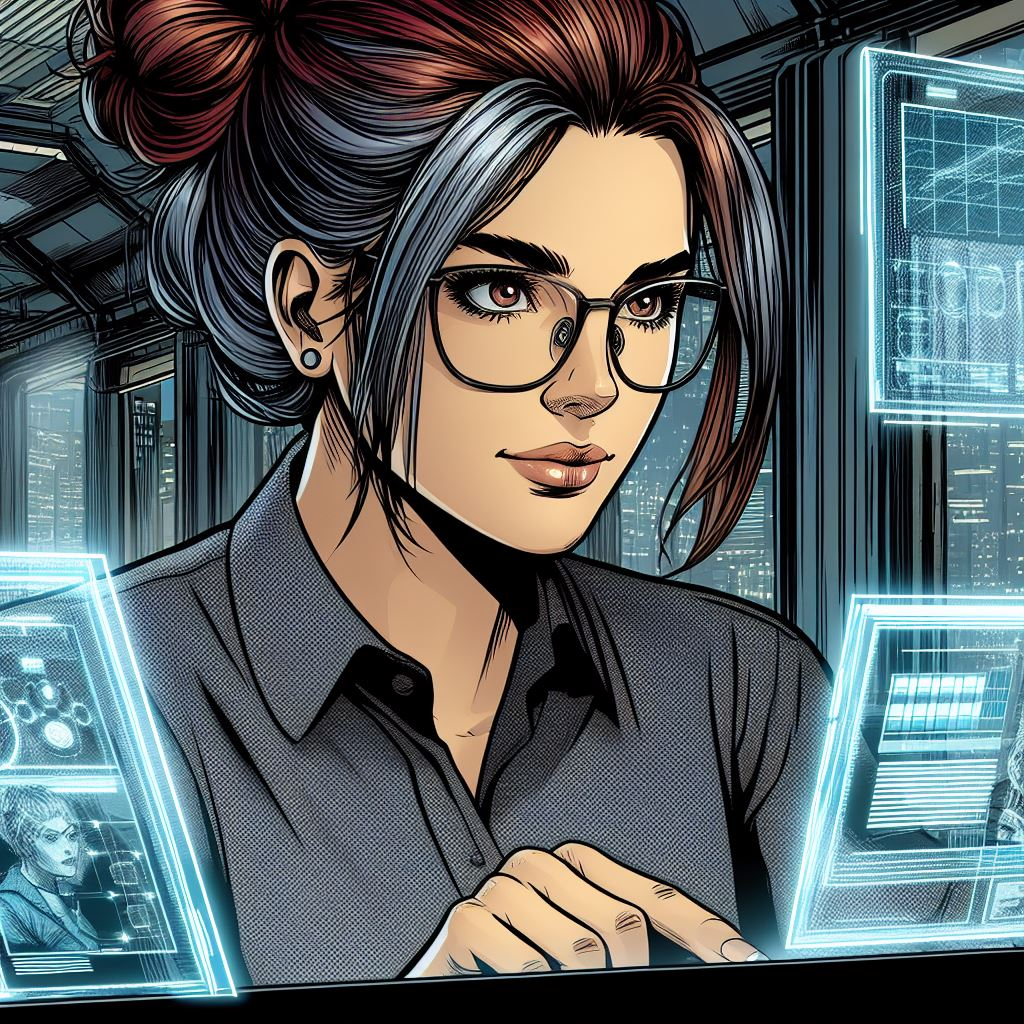
\includegraphics[width=0.6\textwidth]{figures/p2s1.jpeg}
    \caption{Page 2, scene 1 of the comic book.}
    \label{fig:p2s1}
\end{figure}

Since I previously asked a description of the protagonist, I knew that Dr.~Evelyn Hayes is ``a woman in her mid-thirties, with hazel eyes framed by thin-rimmed glasses, chestnut hair streaked with hints of silver, tied in a practical bun''. The prompt I gave to Copilot is the following:
\begin{shadedquotation3}
    \textbf{Me:} A woman in her mid-thirties, with hazel eyes framed by thin-rimmed glasses, chestnut hair streaked with hints of silver, tied in a practical bun, with a focused expression, sits at a sleek workstation in an arcology, examining data on holographic screens. Comic book style. Colored.\smallskip

    \noindent Negative prompt: no black-and-white, no grayscale, no speech bubbles.
\end{shadedquotation3}
Notice that I added some keywords to obtain a correct image:
\begin{itemize}
    \item Comic book style: I wanted the image to be in a comic book style;
    \item Colored: I wanted the image to be colored;
    \item Negative prompt: I wanted to avoid black-and-white and grayscale images, and speech bubbles, which I manually added later.
\end{itemize}
To further obtain consistency, I also added the description of the characters' clothes and the environment, when needed. For example, ``wearing a blouse'', ``wearing a white t-shirt and a brown unbottoned jacket'', ``wearing a spacesuit''. Other important keywords to both achieve consistency and the desired style were ``arcology'', ``futuristic'' and ``holographic screens''.

The images were generated in a few seconds, and I was able to download them directly from the chat. I then manually added the speech bubbles and the narration boxes, and I paginated the comic book using \LaTeX.\medskip

The full text of the prompts for each image is available in the Appendix.

\subsection*{Limitations}
Before setting on using DALL-E 3 integrated into Microsoft Copilot, I tried to use DreamStudio to generate the illustrations. However, there was a major limitation: the AI model was not able to differentiate between the description of two or more characters in a single picture. For example, I wanted a picture depicting both Evelyn and her daughter Lily.

\begin{shadedquotation3}
    \textbf{Me:} In a futuristic arcology, a mother turns to her daughter with a concerned expression, gently placing a hand on her shoulder in an attempt to reassure her. The mother is a woman in her mid-thirties, with hazel eyes framed by thin-rimmed glasses, chestnut hair streaked with hints of silver, tied in a practical bun. The daughter is a girl of about 6 years old with a cherubic face framed by wisps of chestnut hair that cascade in loose curls around her shoulders. Comic book style. Colored.\smallskip 

    \noindent Negative prompt: no black-and-white, no grayscale,  no speech bubbles.
\end{shadedquotation3}

With this prompt I obtained the image in Figure~\vref{fig:distinguish}. As we can see, the daughter's appearance seems to merge with the mother's:  they both wear glasses, and her hair is not curly, but it looks like it's a blend between curls and tied hair. 

\begin{figure}[htb]
    \centering
    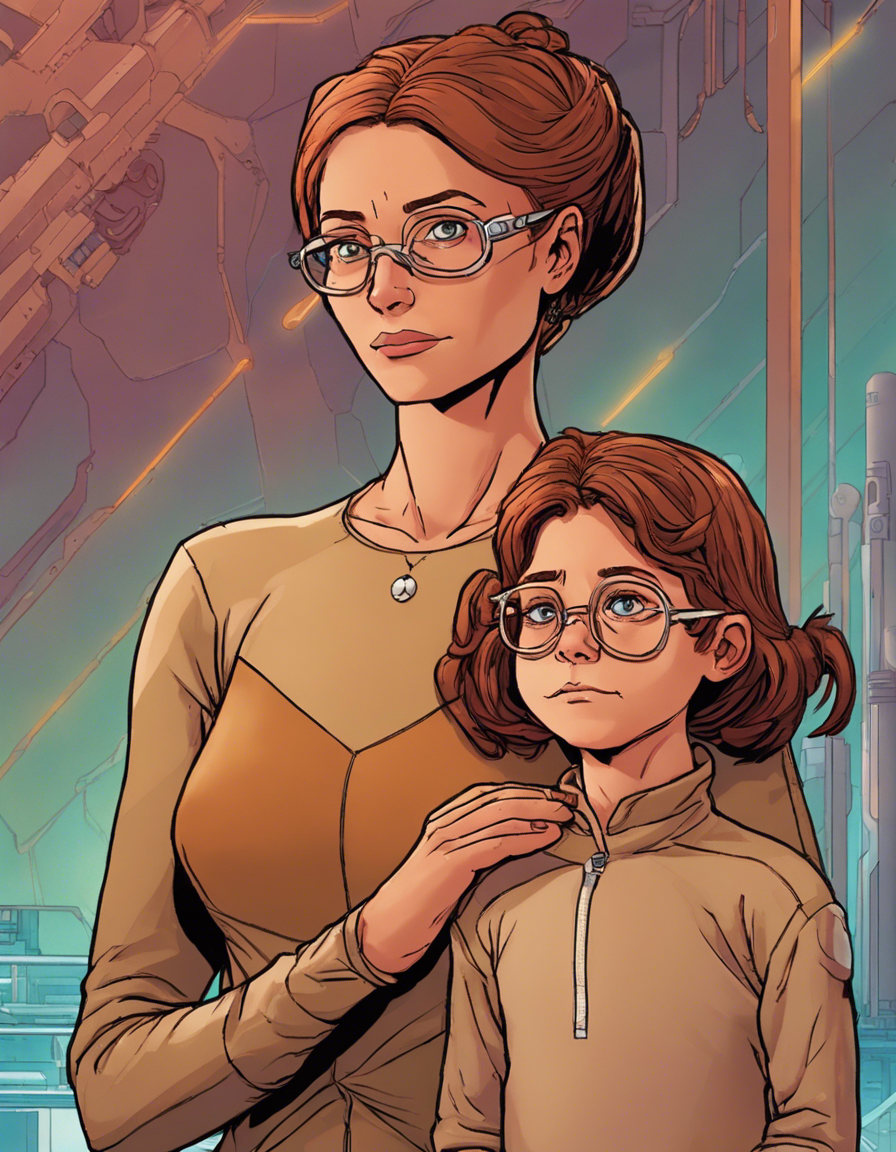
\includegraphics[width=0.6\textwidth]{figures/no-distinguish-between-people.png}
    \caption{Image generated using DreamStudio. I gave the description of two characters, but the AI model was not able to differentiate between them (e.g.~they have the same glasses).}
    \label{fig:distinguish}
\end{figure}

Another thing to look out for is choosing the right keywords when writing the prompt. I already explained which keywords were essential to generate correct images; in Figure~\vref{fig:wrong} there are some examples of wrong prompts and the corresponding output images. Through trial and error I managed to figure out which keywords I had to include (or explicitly exclude) in each prompt to obtain the illustration I wanted. For some panels, this was a time-consuming process, and I had to generate the images multiple times to obtain the desired result.\medskip

\begin{figure}
    \centering
    \begin{subfigure}{0.353\textwidth}
        \begin{subfigure}{1\textwidth}
            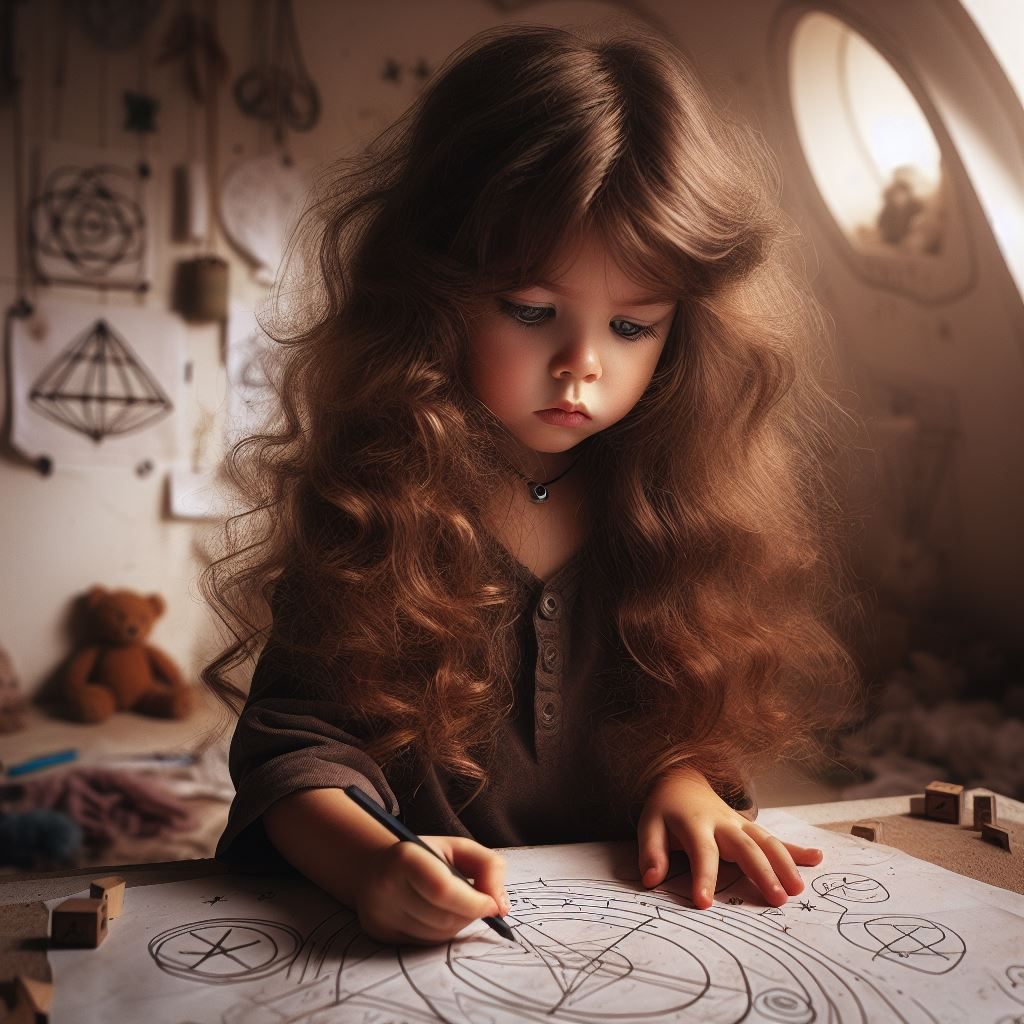
\includegraphics[width=\textwidth]{figures/prompt-1.jpeg}
            \caption{Without ``Comic book style''.}
            % \label{fig:first}
        \end{subfigure}\\
        \begin{subfigure}{1\textwidth}
            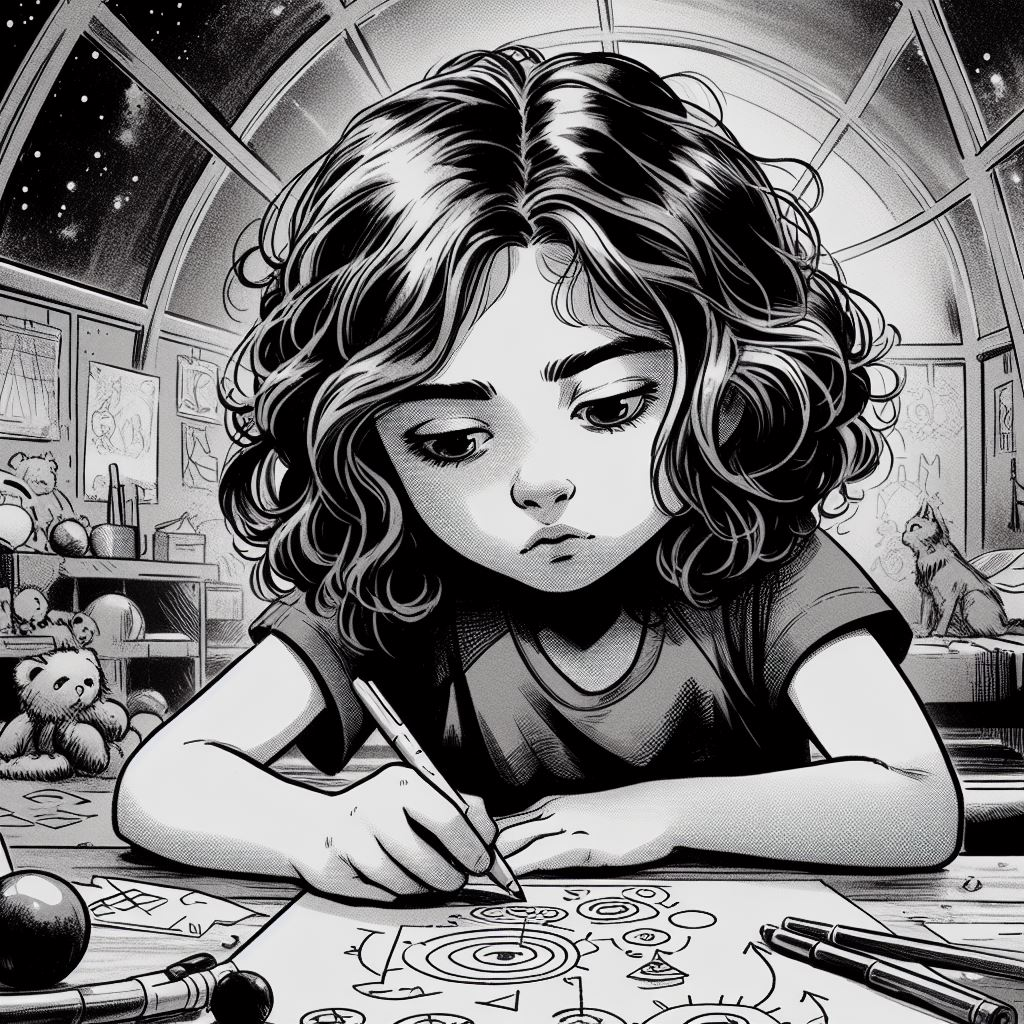
\includegraphics[width=\textwidth]{figures/prompt-2.jpeg}
            \caption{Without ``no balck-and-white, no grayscale''.}
            % \label{fig:second}
        \end{subfigure}
    \end{subfigure}
    \hfill
    \begin{subfigure}{0.6\textwidth}
        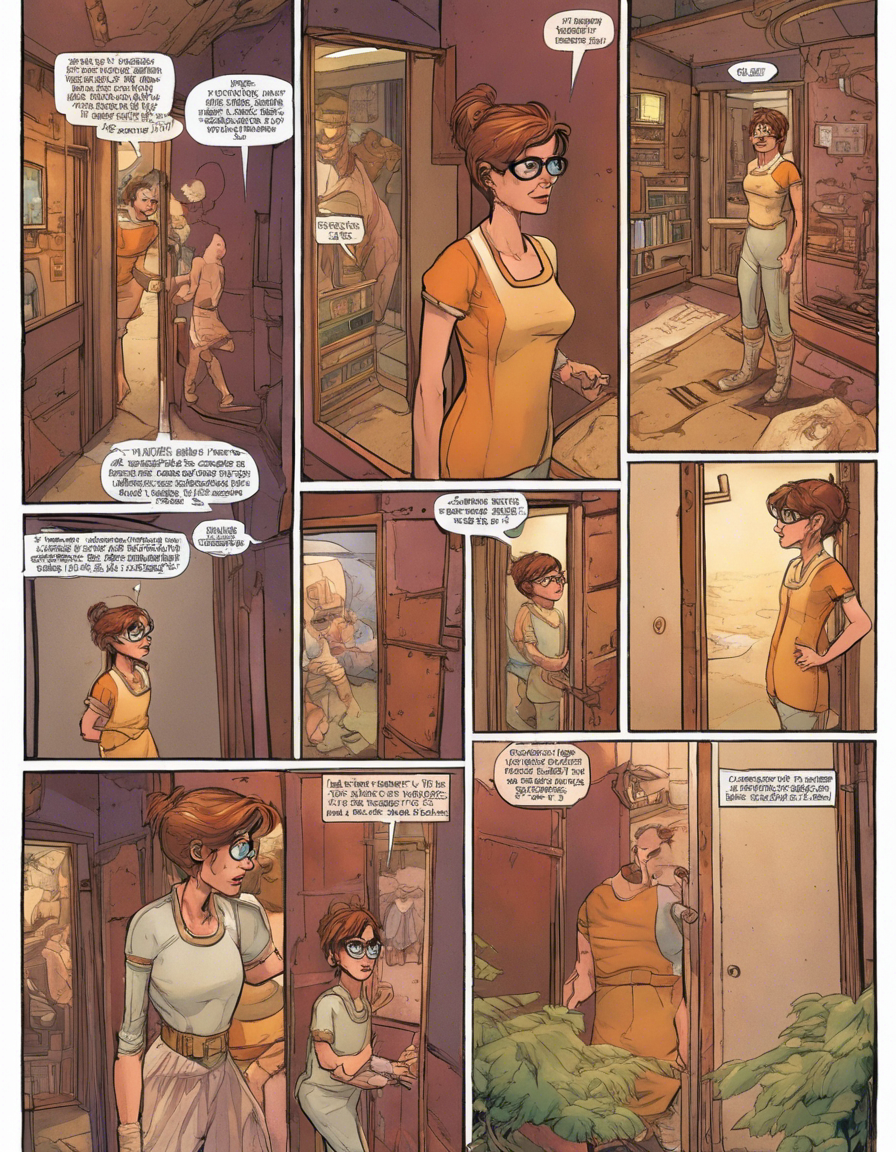
\includegraphics[width=\textwidth]{figures/without-negative-prompt-1.png}
        \caption{Without ``no speech bubbles''.}
        % \label{fig:third}
    \end{subfigure}
            
    \caption{Examples of images generated without important keywords.}
    \label{fig:wrong}
\end{figure}

I also ``stress-tested'' the AI model by asking it to generate a picture over and over. Specifically, I used the following prompt:
\begin{shadedquotation3}
    \textbf{Me:} Comic book style. A girl of about 6 years old with a cherubic face framed by wisps of chestnut hair that cascade in loose curls around her shoulders sits in her quarters in an arcology, surrounded by toys and drawings scattered across the floor. She is deeply engrossed in drawing mysterious symbols on a sheet of paper, her brow furrowed in concentration as she works.\smallskip 

    \noindent Negative prompt: no black-and-white, no grayscale,  no speech bubbles.
\end{shadedquotation3}

By doing this, I discovered a possible bias of the model: the majority of the generated images were of a caucasian girl, and only in 2 cases out of dozens I was able to obtain a picture of a girl with a different ethnicity (Fig~\vref{fig:bias}).\medskip

\begin{figure}
    \centering
    \begin{subfigure}{0.6\textwidth}
        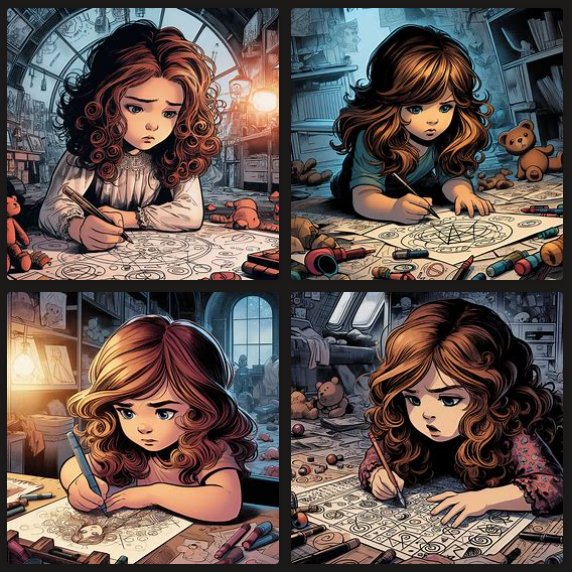
\includegraphics[width=\textwidth]{figures/caucasian.png}
    \end{subfigure}
    \hfill 
    \begin{subfigure}{0.353\textwidth}
        \begin{subfigure}{1\textwidth}
            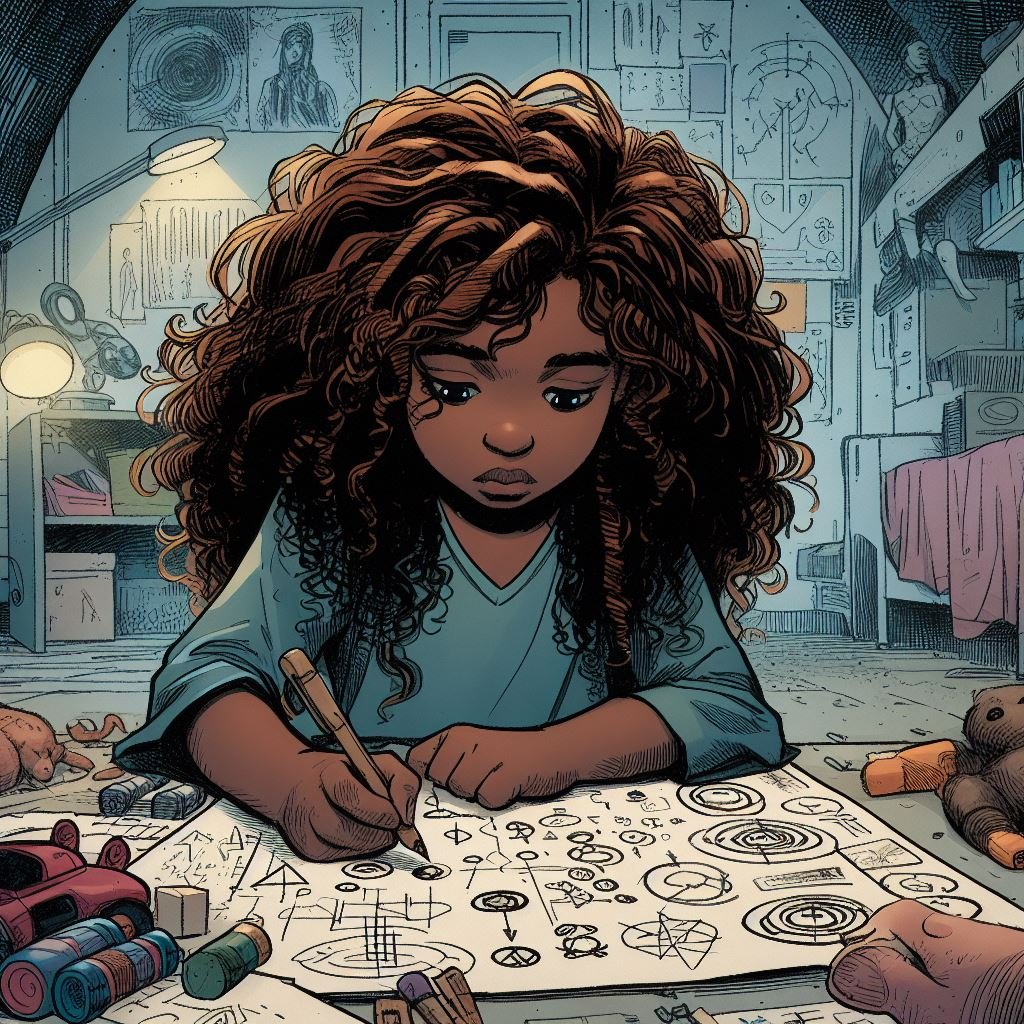
\includegraphics[width=\textwidth]{figures/bias.jpeg}
        \end{subfigure}\\
        \begin{subfigure}{1\textwidth}
            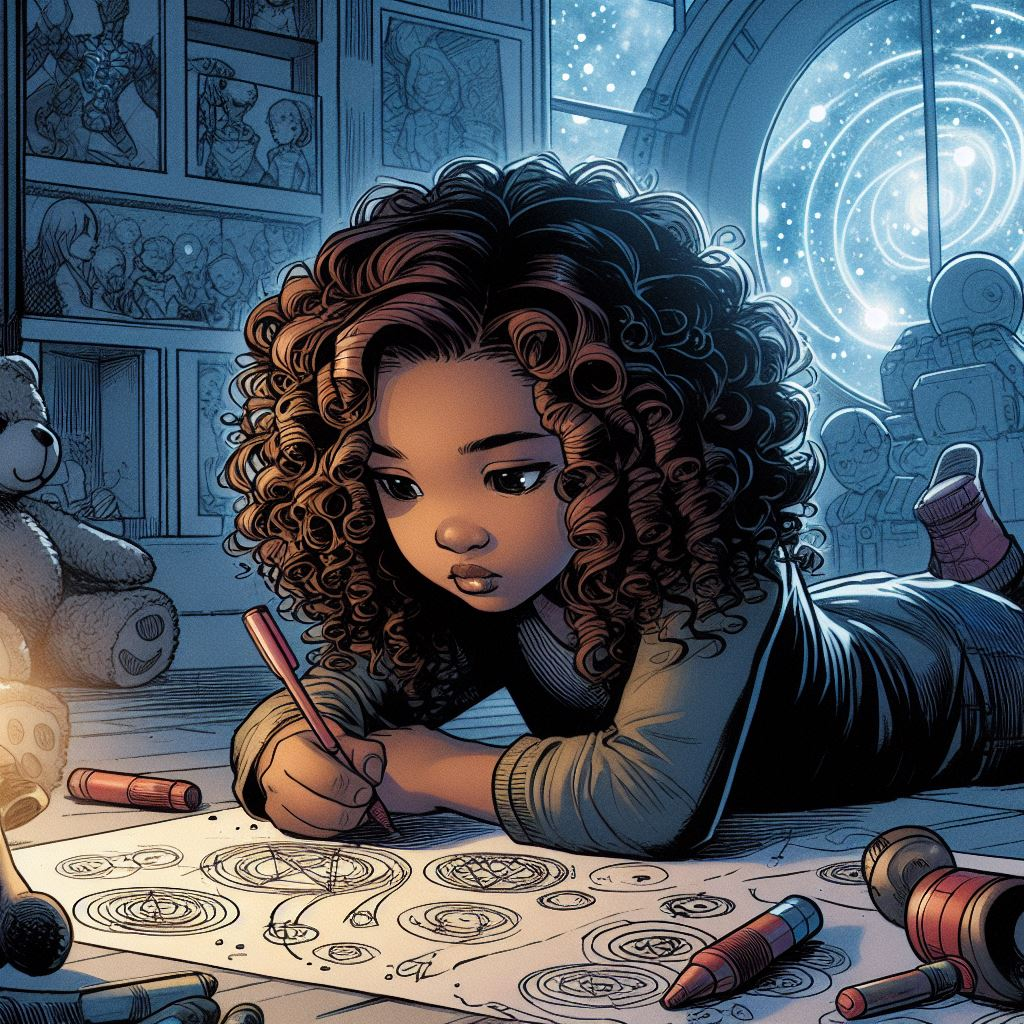
\includegraphics[width=\textwidth]{figures/bias2.jpeg}
        \end{subfigure}
    \end{subfigure}
            
    \caption{When describing a girl without specifying the ethnicity, the AI model generated, in the majority of cases, a caucasian girl (left). Only in 2 cases out of dozens I was able to obtain a picture of a girl with a different ethnicity (right).}
    \label{fig:bias}
\end{figure}

Finally, I initially could not generate images of Lily. When giving to different AI models her description, I was met with error messages, such as ``Something isn't quite right with your prompts''. By tweaking and changing the description, I was able to bot obtain the images I wanted and understand what was wrong with the prompt: I was using words like ``young girl'' or ``little girl'', which I understand might be problematic. By changing the description to ``A girl of about 6 years old'' I was able to bypass this limitation.



%%%%%%%%%%%%%%%%%%%%%%
\newpage
\section{Conclusions}
In this report, I illustrated how I generated a short comic book story using free online generative AI tools. I found that the generative AI tools I used were effective in generating the story and the illustrations, but they also have some limitations.

In conclusion, I believe that generative AI tools can be effectively used to generate a short comic book story, but they also have some constraints that need to be taken into account. I also believe that the limitations I encountered could be addressed by further refining the prompts and by using different tools. 





\newpage
\appendix

%%%%%%%%%%%%%%%%%%%%%%
\section{Appendix: Text Prompts}



%%%%%%%%%%%%%%%%%%%%%%
\newpage
\section{Appendix: Image Prompts}


\newpage 
\bibliographystyle{plain} 
\bibliography{references} 


\end{document}